\documentclass[12pt, twoside]{book}
%\documentclass[12pt, oneside]{book}  % jednostranna tlac

%spravne nastavenie okrajov
\usepackage[a4paper,top=2.5cm,bottom=2.5cm,left=3.5cm,right=2cm]{geometry}
%zapnutie fontov pre UTF8 kodovanie
\usepackage[utf8]{inputenc}
\usepackage[T1]{fontenc}
\usepackage{textgreek}

%zapnutie slovenskeho delenia slov
%a automatickych nadpisov ako Obsah, Obrázok a pod. v slovencine
%\usepackage[slovak]{babel} % vypnite pre prace v anglictine!

%nastavenie riadkovania podla smernice
\linespread{1.25} % hodnota 1.25 by mala zodpovedat 1.5 riadkovaniu

% balicek na vkladanie zdrojoveho kodu
\usepackage{listings}
% ukazky kodu su cislovane ako Listing 1,2,...
% tu je Listing zmenene na Algoritmus 1,2,...
\renewcommand{\lstlistingname}{Algoritmus}
% nastavenia balicka listings
% mozete pridat aj language=...
% na nastavenie najcastejsie pouzivaneho prog. jazyka
% takisto sa da zapnut cislovanie riadkov
\lstset{frame=lines}

% balicek na vkladanie obrazkov
\usepackage{graphicx}
% balicek na spravne formatovanie URL
\usepackage{url}
% balicek na hyperlinky v ramci dokumentu
% zrusime farebne ramiky okolo liniek aby pdf
% vyzeralo rovnako ako tlacena verzia
\usepackage[hidelinks,breaklinks]{hyperref}


% -------------------
% --- Definicia zakladnych pojmov
% --- Vyplnte podla vasho zadania
% -------------------
\def\mfrok{2022}
\def\mfnazov{An end-to-end pipeline for detection of endolysin proteins from raw sequencing reads}
\def\mftyp{Bachelor Thesis}
\def\mfautor{Juraj Vašut}
\def\mfskolitel{MSc. Andrej Baláž}

%ak mate konzultanta, odkomentujte aj jeho meno na titulnom liste
\def\mfkonzultant{tit. Meno Priezvisko, tit. }  

\def\mfmiesto{Bratislava, \mfrok}

% bioinformatici odkomentujú riadok s dvoma odbormi a iný program
%\def\mfodbor{Computer Science}
\def\mfodbor{Computer Science and Biology} 
%\def\program{Computer Science }
\def\program{ Bioinformatics }

% Ak je školiteľ z FMFI, uvádzate katedru školiteľa, zrejme by mala byť aj na zadaní z AIS2
% Ak máte externého školiteľa, uvádzajte Katedru informatiky 
\def\mfpracovisko{ Department of Applied Informatics }

\begin{document}     
\frontmatter


% -------------------
% --- Obalka ------
% -------------------
\thispagestyle{empty}

\begin{center}
  \sc\large
  Comenius University in Bratislava\\
  Faculty of Mathematics, Physics and Informatics

\vfill

{\LARGE\mfnazov}\\
\mftyp
\end{center}

\vfill

{\sc\large 
\noindent \mfrok\\
\mfautor
}

\cleardoublepage
% --- koniec obalky ----

% -------------------
% --- Titulný list
% -------------------

\thispagestyle{empty}
\noindent

\begin{center}
\sc  
\large
  Comenius University in Bratislava\\
  Faculty of Mathematics, Physics and Informatics

\vfill

{\LARGE\mfnazov}\\
\mftyp
\end{center}

\vfill

\noindent
\begin{tabular}{ll}
Study Programme: & \program \\
Field of Study: & \mfodbor \\
Department: & \mfpracovisko \\
Supervisor: & \mfskolitel \\
% Consultant: & \mfkonzultant \\
\end{tabular}

\vfill


\noindent \mfmiesto\\
\mfautor

\cleardoublepage
% --- Koniec titulnej strany


% -------------------
% --- Zadanie z AIS
% -------------------
% v tlačenej verzii s podpismi zainteresovaných osôb.
% v elektronickej verzii sa zverejňuje zadanie bez podpisov
% v pracach v naglictine anglicke aj slovenske zadanie

\newpage 
\thispagestyle{empty}
\hspace{-2cm}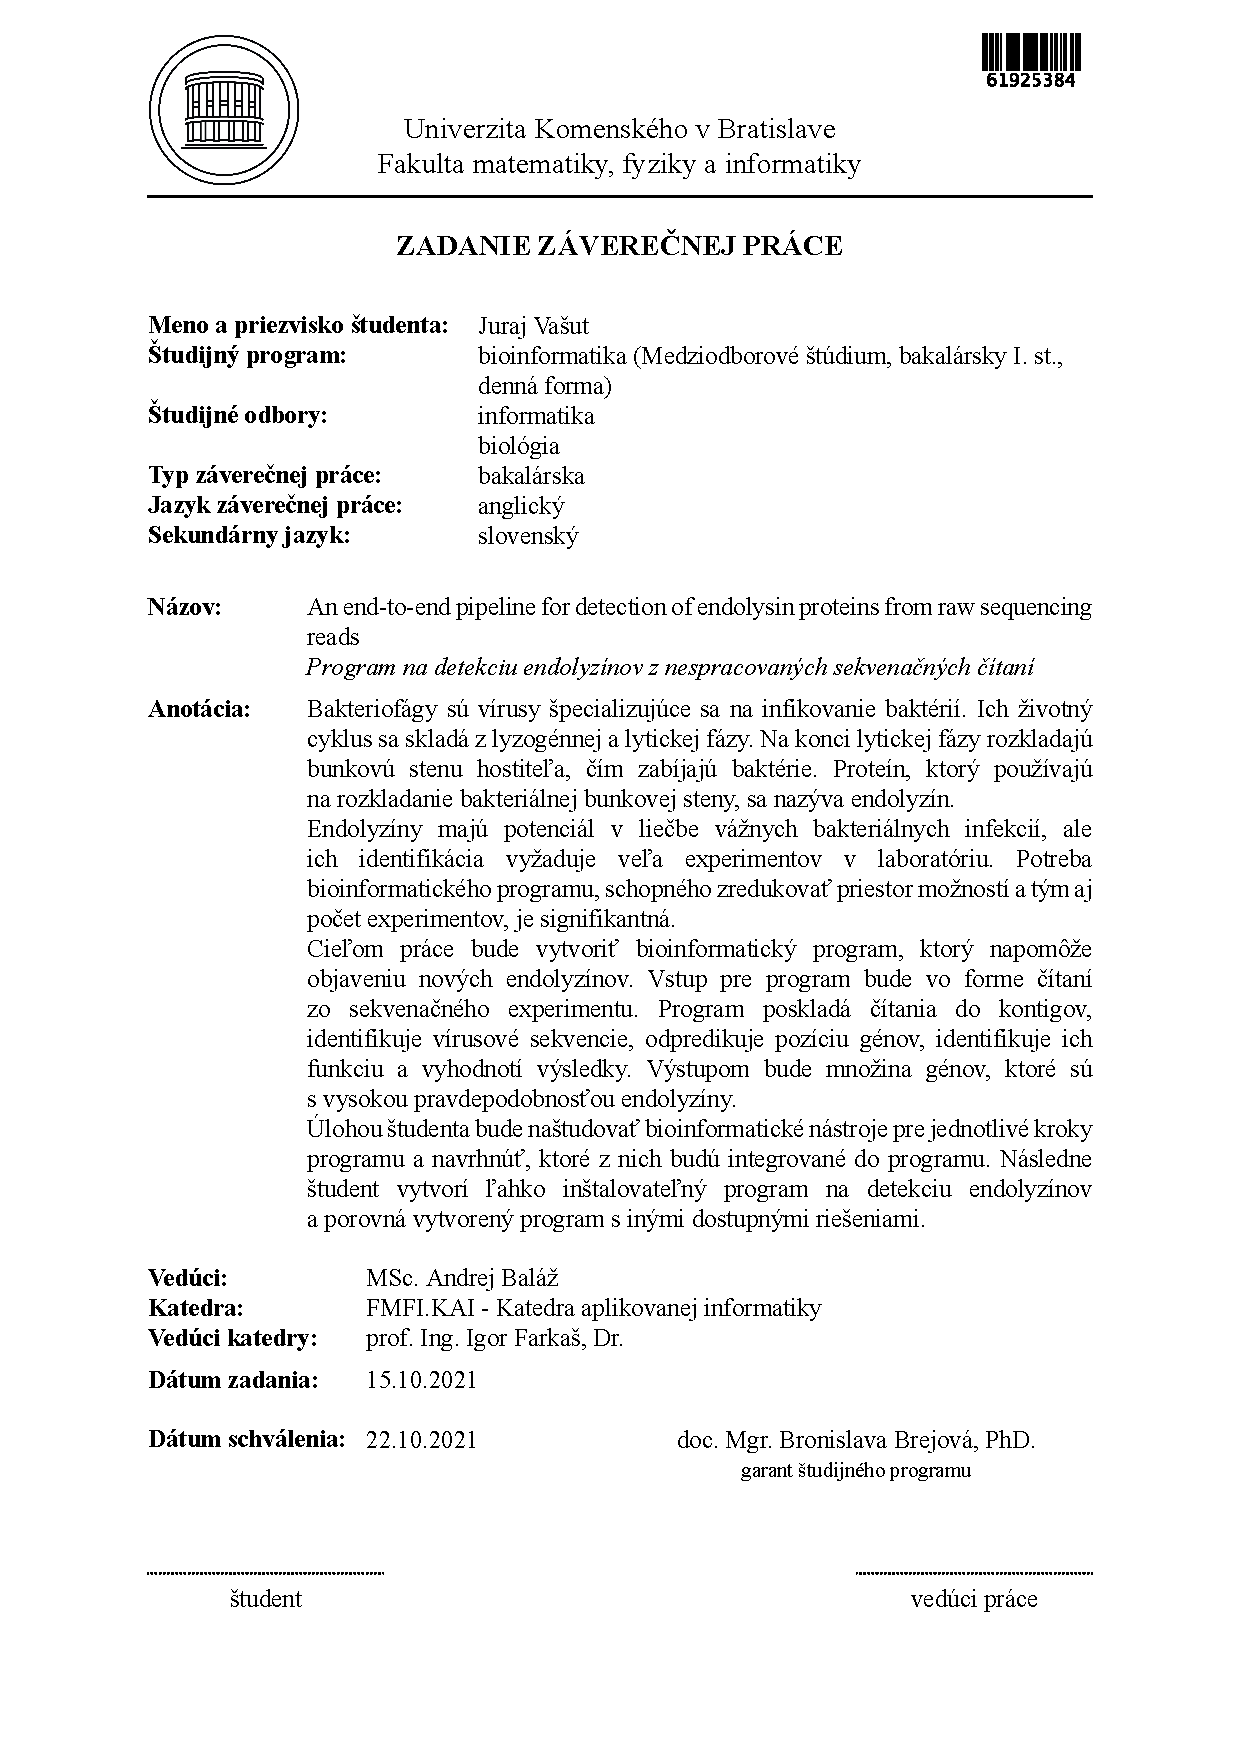
\includegraphics[width=1.1\textwidth]{images/zadanie}

\hspace{-2cm}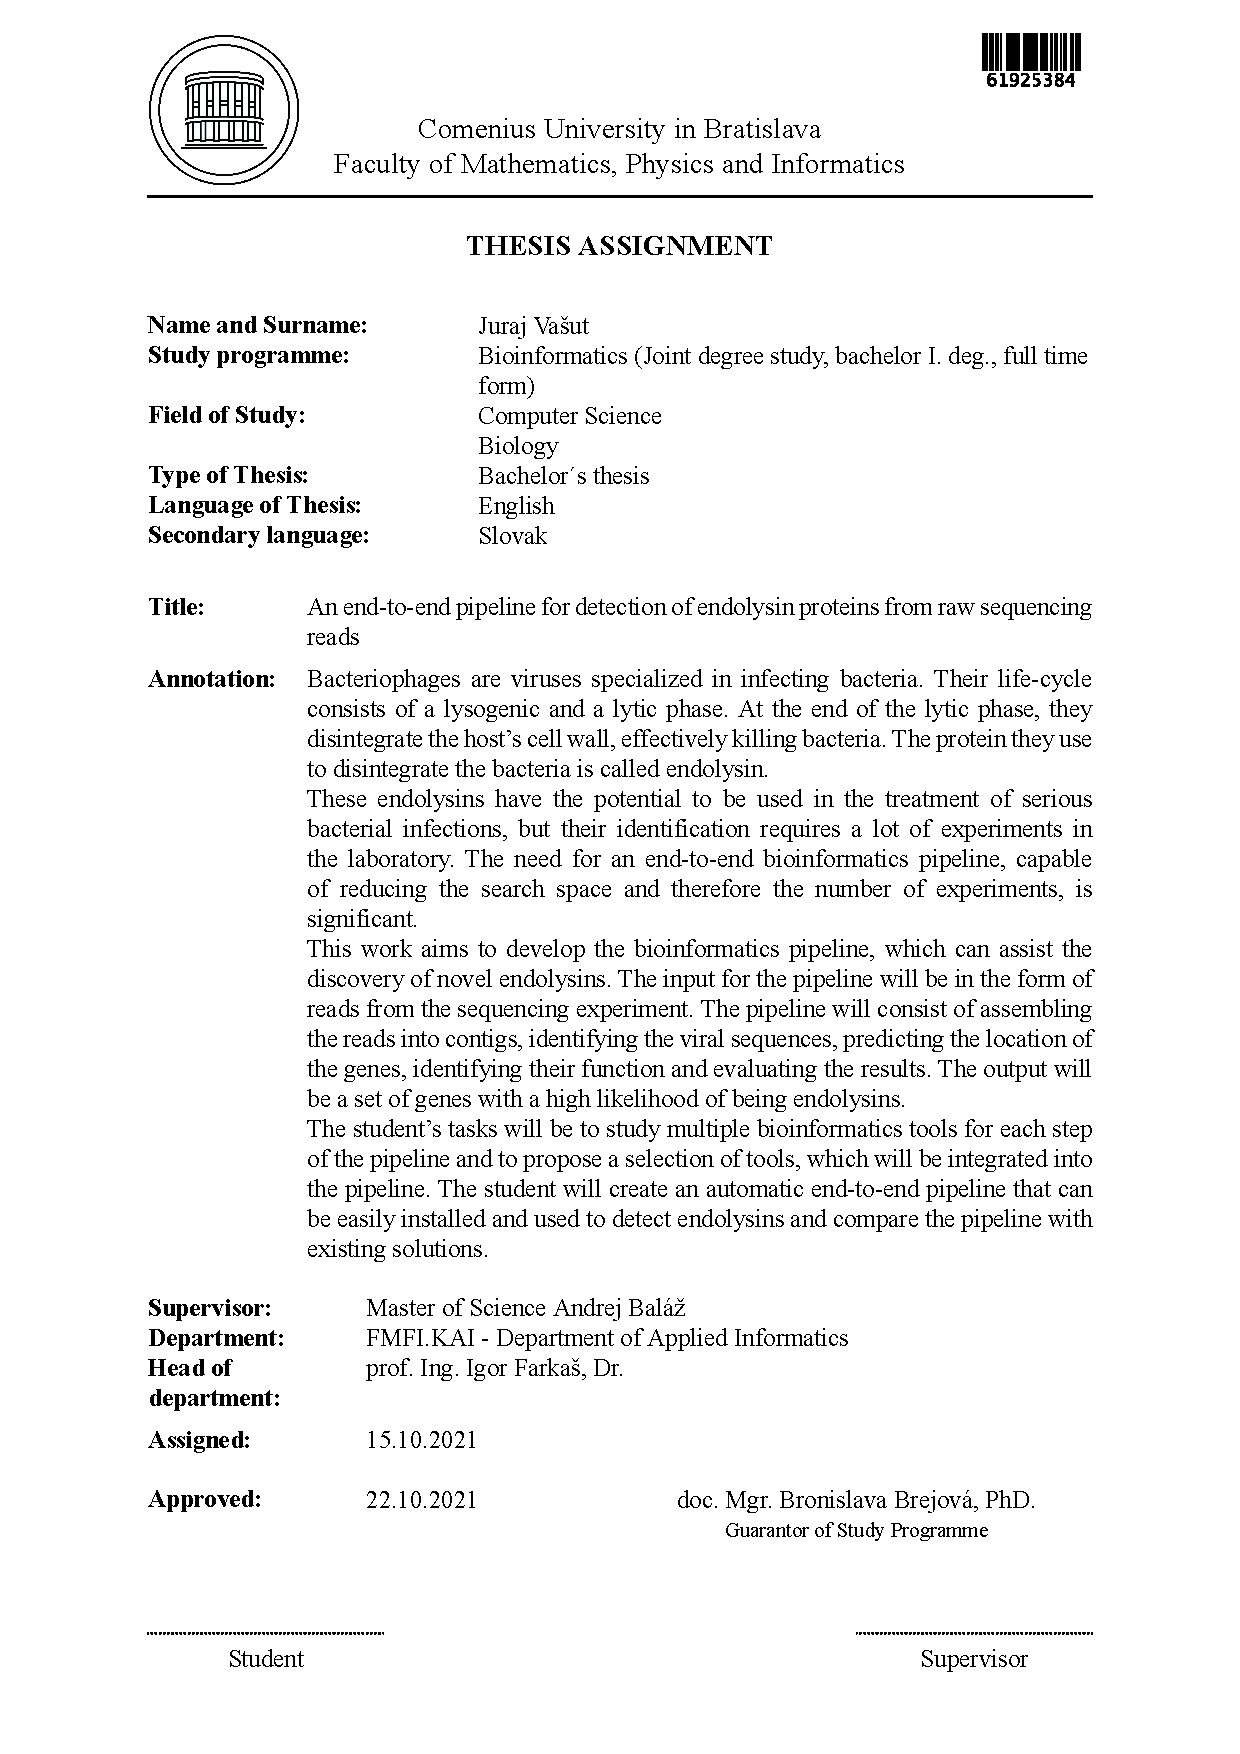
\includegraphics[width=1.1\textwidth]{images/zadanie-en}

% --- Koniec zadania

\frontmatter

% -------------------
%   Poďakovanie - nepovinné
% -------------------
\setcounter{page}{3}
\newpage 

\vfill
{\bf Acknowledgments:} 

% --- Koniec poďakovania

% -------------------
%   Abstrakt - Slovensky
% -------------------
\newpage 
\section*{Abstrakt}
\paragraph*{}
Nadmerné používanie antibiotík viedlo k vývoju multirezistentných baktérií. Tieto baktérie sú odolné voči veľkému množstvu antibiotík, čo sťažuje liečbu infekcií nimi spôsobenými. Z tohto dôvodu sa vyvíjajú ďalšie metódy liečby bakteriálnych infekcií. Jednou z metód je fágová terapia zahŕňajúca použitie bakteriofágových endolyzínov na zacielenie na konkrétne baktérie. Kvôli nedostatku nástrojov navrhnutých na analýzu vírusových genómov si objavovanie nových endolyzínov vyžaduje použitie zložitých zreťazených spracovávaní s veľkým počtom krokov. Aby sme uľahčili objavenie nových endolyzínov, predstavujeme jednoduchý nástroj Phendol schopný presne predpovedať endolyzíny v nespracovaných párovaných sekvenčných čítaniach.

\paragraph*{Kľúčové slová:} endolyzín, anotácia génov, baktériofág, skladanie kontigov, zreťazené spracovanie
% --- Koniec Abstrakt - Slovensky


% -------------------
% --- Abstrakt - Anglicky 
% -------------------
\newpage 
\section*{Abstract}
\paragraph*{}
The overuse of antibiotics has led to the evolution of multiresistant bacteria. These bacteria are resistant to a large number of antibiotics, making the infections caused by them more difficult to cure. For this reason, other methods to cure bacterial infections are being developed. One of the methods is phage therapy involving the use of bacteriophage endolysins to target specific bacteria. Due to the lack of tools designed for analysis of viral genomes, the discovery of new endolysins requires use of complex pipelines with a large number of steps involved. To facilitate an easier discovery of new endolysins, we introduce a simple end-to-end pipeline Phendol capable of accurate prediction of endolysins in raw paired end sequencing reads.

\paragraph*{Keywords:} endolysin, gene annotation, bateriophage, contig assembly, pipeline

% --- Koniec Abstrakt - Anglicky

% -------------------
% --- Predhovor - v informatike sa zvacsa nepouziva
% -------------------
%\newpage 
%\thispagestyle{empty}
%
%\huge{Predhovor}
%\normalsize
%\newline
%Predhovor je všeobecná informácia o práci, obsahuje hlavnú charakteristiku práce 
%a okolnosti jej vzniku. Autor zdôvodní výber témy, stručne informuje o cieľoch 
%a význame práce, spomenie domáci a zahraničný kontext, komu je práca určená, 
%použité metódy, stav poznania; autor stručne charakterizuje svoj prístup a svoje 
%hľadisko. 
%
% --- Koniec Predhovor


% -------------------
% --- Obsah
% -------------------

\newpage 

\tableofcontents

% ---  Koniec Obsahu

% -------------------
% --- Zoznamy tabuliek, obrázkov - nepovinne
% -------------------

\newpage 

\listoffigures
\listoftables

% ---  Koniec Zoznamov

\mainmatter


\input uvod.tex 

%\input kapitola.tex

%\input latex.tex

%\input lorem.tex

%\chapter{A Sample Text}
%Chapters in Slovak language are commented out, but use them as a guide
%to write chapters in English. Here we only cite some references, such
%as a book about LaTeX \cite{Oetiker2000}, a scientific journal article
%\cite{clanok}, a conference paper \cite{clanok_na_konferencii}, a
%technical report \cite{technical_report}, a book \cite{kniha}, and a
%resourse from the Internet \cite{smernica}.

\input kapitola1.tex
\input kapitola2.tex
\input kapitola3.tex
\input kapitola4.tex
%\input kapitola.tex

\input zaver.tex

% -------------------
% --- Bibliografia
% -------------------


\newpage	

\backmatter

\thispagestyle{empty}
\clearpage

\bibliographystyle{plain}
\bibliography{literatura} 

%Prípadne môžete napísať literatúru priamo tu
%\begin{thebibliography}{5}
 
%\bibitem{br1} MOLINA H. G. - ULLMAN J. D. - WIDOM J., 2002, Database Systems, Upper Saddle River : Prentice-Hall, 2002, 1119 s., Pearson International edition, 0-13-098043-9

%\bibitem{br2} MOLINA H. G. - ULLMAN J. D. - WIDOM J., 2000 , Databasse System implementation, New Jersey : Prentice-Hall, 2000, 653s., ???

%\bibitem{br3} ULLMAN J. D. - WIDOM J., 1997, A First Course in Database Systems, New Jersey : Prentice-Hall, 1997, 470s., 

%\bibitem{br4} PREFUSE, 2007, The Prefuse visualization toolkit,  [online] Dostupné na internete: <http://prefuse.org/>

%\bibitem{br5} PREFUSE Forum, Sourceforge - Prefuse Forum,  [online] Dostupné na internete: <http://sourceforge.net/projects/prefuse/>

%\end{thebibliography}

%---koniec Referencii

% -------------------
%--- Prilohy---
% -------------------

%Nepovinná časť prílohy obsahuje materiály, ktoré neboli zaradené priamo  do textu. Každá príloha sa začína na novej strane.
%Zoznam príloh je súčasťou obsahu.
%
%\input appendixA.tex

%\input appendixB.tex

\end{document}






